

\tikzset{every picture/.style={line width=0.75pt}} %set default line width to 0.75pt        

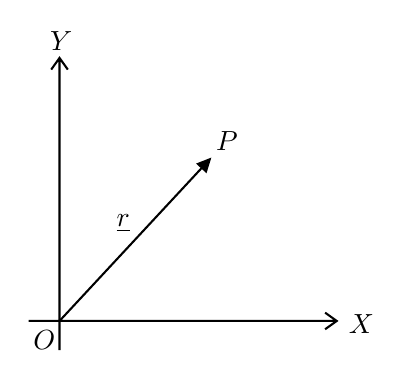
\begin{tikzpicture}[x=0.75pt,y=0.75pt,yscale=-0.8,xscale=0.8]
%uncomment if require: \path (0,300); %set diagram left start at 0, and has height of 300

%Shape: Axis 2D [id:dp15761041967637524] 
\draw  (150,228.4) -- (335.5,228.4)(168.55,70) -- (168.55,246) (328.5,223.4) -- (335.5,228.4) -- (328.5,233.4) (163.55,77) -- (168.55,70) -- (173.55,77)  ;
%Straight Lines [id:da5719661880478002] 
\draw    (168.55,228.4) -- (257.96,132.2) ;
\draw [shift={(260,130)}, rotate = 492.9] [fill={rgb, 255:red, 0; green, 0; blue, 0 }  ][line width=0.08]  [draw opacity=0] (8.93,-4.29) -- (0,0) -- (8.93,4.29) -- cycle    ;

% Text Node
\draw (151,232.4) node [anchor=north west][inner sep=0.75pt]    {$O$};
% Text Node
\draw (261,112.4) node [anchor=north west][inner sep=0.75pt]    {$P$};
% Text Node
\draw (161,52.4) node [anchor=north west][inner sep=0.75pt]    {$Y$};
% Text Node
\draw (341,222.4) node [anchor=north west][inner sep=0.75pt]    {$X$};
% Text Node
\draw (201,162.4) node [anchor=north west][inner sep=0.75pt]    {$\underline{r}$};


\end{tikzpicture}